\documentclass[11pt,a4paper]{article}

\usepackage{url,,}
\usepackage{graphicx}
\usepackage{hyperref}
\usepackage{amsfonts}
\usepackage{amssymb}
\usepackage{amsmath}
\usepackage{amsfonts}
\usepackage{amssymb}
\usepackage{amsmath}
\usepackage{multirow}
\usepackage{listings}
\usepackage{fullpage}
\usepackage{fancyhdr,a4wide}
\usepackage{makeidx}
\usepackage{placeins}
\usepackage[procnames,noindent]{lgrind}

\lstset{ %
language=VHDL,                % choose the language of the code
basicstyle=\footnotesize,       % the size of the fonts that are used for the code
showstringspaces=false,         % underline spaces within strings
%numbers=left,                   % where to put the line-numbers
%numberstyle=\footnotesize,      % the size of the fonts that are used for the line-numbers
%stepnumber=1,                   % the step between two line-numbers. If it's 1 each line will be numbered
%numbersep=5pt,                  % how far the line-numbers are from the code
%backgroundcolor=\color{white},  % choose the background color. You must add \usepackage{color}
showspaces=false,               % show spaces within strings adding particular underscores
showtabs=false,                 % show tabs within strings adding particular underscores
escapeinside={\%*}{*)}          % if you want to add a comment within your code
}

\begin{document}	

\begin{titlepage}

\thispagestyle{fancy}
\lhead{}
\chead{
\large{\textit{
Informatics and Mathematical Modelling\\
Technical University of Denmark}}}
\rhead{}
\rule{0pt}{50pt}
\vspace{3cm}

\begin{center}

 	\huge{\textbf{02207 : Advanced Digital Design Techniques}}\\
 	\vspace{1cm}
 	\huge{Exercise of Retiming}\\
 	\vspace{1cm}
 	\huge{\textit{LAB 3}}\\
 	\vspace{1cm}
 	\huge{Group \textit{dt07}}\\
\end{center}

\vspace{4cm}

\begin{flushright}
	\LARGE{Markku Eerola (s053739)}\\
	\vspace{0.3cm}
	\LARGE{Rajesh Bachani (s061332)}\\
	\vspace{0.3cm}
	\LARGE{Josep Renard (s071158)}\\
\end{flushright}
\cfoot{\today}
\end{titlepage}

%\begin{abstract}
%\centering
%Abstract to be created.
%\end{abstract}

%-----------------------------------------------------------
\newpage 
\tableofcontents

\newpage 
% --- I thought about a different document structure which I feel would be more natural. I removed the subsections from the introduction and added the cell counts and dissipated power into the sections about the designs. Read it through and think which you prefer.

\section{Introduction}
This document is report of the third exercise on DTU course Advanced Digital Design. In this exercise we studied the concept of retiming using a digit recurrence division implementation with radix-4 and carry-save adder.

In course of the exercise we examined two designs, the original design for digit recurrence division and the retimed design. We first compiled, simulated and synthesized the original design to get the power report and cell counts for it. We then modified the VHDL code for the original design to retime the recurrence. This retimed design was then also compiled, simulated and synthesized to get the power report and cell counts.

In the following sections we will briefly explain the concept of retiming, present the original circuit and the retimed circuit and the power dissipated and cells used in both. In the last section we will discuss the results.

\subsection{Authors by Section}
\begin{itemize}
\item \textit{Rajesh Bachani} 
\item \textit{Josep Renard} 
\item \textit{Markku Eerola} 
\end{itemize}

\section{Retiming}
Retiming is an optimizing technique where structural location of registers is manually moved without affecting the functionality of the circuit in order to improve its performance. This is done either by removing a register from each input to a block and adding a register to each output, or by adding registers to the inputs and removing registers from the outputs.

In our case the motivation for retiming was to create slack on a non-critical path, and to have the synthesizer substitute HS cells with LL cells on this path thus lowering the overall power dissipation in the whole circuit. According to the lecture slides the circuit we were studying should gain approximately 30\% power savings from this kind of retiming.

\section{Original Design}
The original design upon which we aimed to improve with the retiming is presented in figure 1.

\begin{figure}
	\centering
		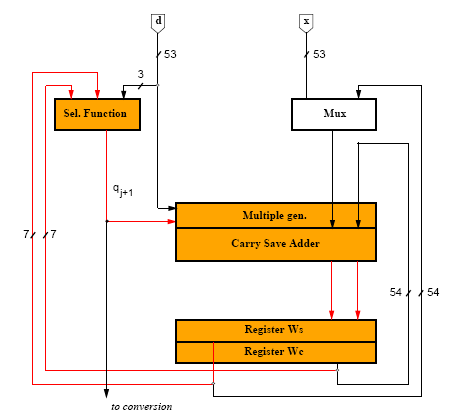
\includegraphics[width=4in]{./noretiming.PNG}
	\caption{Digit recurrence division}	\label{fig:noretiming}
\end{figure}

\FloatBarrier

The Sel. function -block implements the quotient digit selection function. The selection function determines a 4-bit quotient digit using 3 most significant bits of the divisor d and 7 most significant bits from the results stored in registers Ws and Wc.

The MUX block selects the input for the divisor multiplication between the dividend, which is used only in the initialization phase of the division algorithm, and the result of the substraction of the quotient digit/divisor multiplication result from the dividend. The substraction result is stored in register Ws.

The Multiple gen. -block implements the divisor multiplication ie. it multiplies the divisor d with the 4-bit quotient digit. This block is basically a multiplexer.

The Carry Save Adder -block implements the substraction of the result of the divisor multiplication from the dividend. The substraction is done with a carry-save adder as the name of the block suggests.

The registers Ws and Wc store the carry and the sum from the carry-save adder respectively.

The critical path of this circuit is marked with red arrows in the figure 1.

\subsection{Power dissipation and cell count}
The Synopsys VSS Simulator was used to annotate the switching activity based on a testbench and test vectors. This switching activity was used by Design Vision to estimate the power dissipation within the circuit. The results can be seen in table 1 for each composing block. The actual report is in appendix A.

The table also shows the number of HVT and SVT cells in each composing block.

% ----------------------------------------------------- Which component does Control belong to? Mux?
\begin{table}[htbp]
\caption{Power dissipation in original circuit (uW) and cell count}
\begin{center}
\begin{tabular}{|l|l|l|l|l|l|} % I don't know if this is the correct way, I was just guessing from what I saw in the lab2 tex file
\hline
\textbf{Block}	& \textbf{P static}		& \textbf{P dynamic}	& \textbf{P total} & \textbf{SVT cells} & \textbf{HVT cells}\\ \hline
Mux & 0.12 & 28.3 & 28.4 & 1 & 57 	\\ \hline
Mult. gen. & 6.8 & 124.0 & 130.8 & 226 & 51 	\\ \hline
CSA & 7.4 & 196.4 & 203.8 & 141 & 35 	\\ \hline
SEL & 3.3 & 68.1 & 71.4 & 80 & 5 	\\ \hline
Reg W & 13.3 & 336.7 & 350.0 & 315 & 8 	\\ \hline
\end{tabular}
\end{center}
\label{table:powerOriginal}
\end{table}


\section{Retimed Design}
The retimed design is presented in figure 2.

\begin{figure}
	\centering
		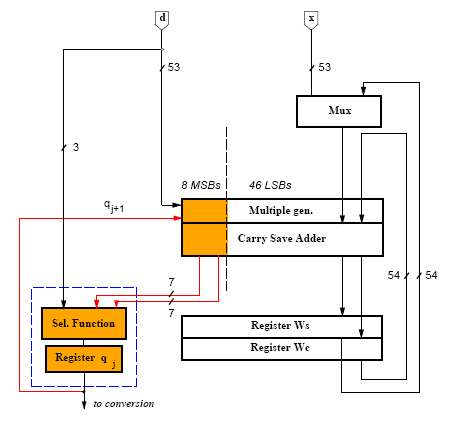
\includegraphics[width=4in]{./retiming.PNG}
	\caption{Digit recurrence division retimed}
	\label{fig:retiming}
\end{figure}

\FloatBarrier

Since only the most significant bits of sum and carry are used in the quotient digit selection it makes sense to separate the most significant bits from the least significant bits to separate structural slices. This is done in the VHDL code by disconnecting the quotient digit selection block from the W registers thus \textit{removing registers from the inputs} and adding new registers to the output of the block. This frees the W registers from the most significant slice. By also separating the implementation of the most significant bits of the adder and the multiplie generation from the implementation for the less significant bits more of the design is freed from the critical path.

We achieved these changes by editing the top-level VHDL file for the original design. We disconnected the higher bits of register W from the selection function and introduced the register q as a new component. We connected the high bits of CSA directly to the selection function and connected the new register between the selection and the multiple generation.

These changes do not affect the functionality of the circuit, but by dividing the implementation to most significant and least significant slices we get two paths. The critical path is marked with red arrows in the figure 2. The delay on the critical path is T(SEL)+T(reg q)+T(mux)+T(CSA). The delay on the non-critical path is at maximum T(reg W)+T(mux)+T(CSA). From this it can be seen that the non critical path has some slack which the synthesizer should be able to use to optimize the least significant slice for power, namely by replacing HS cells with LL cells.

\subsection{Power dissipation and cell count}
Just as with the original design the Synopsys VSS Simulator was used to annotate the switching activity based on a testbench and test vectors. This switching activity was again used by Design Vision to estimate the power dissipation within the circuit. The results can be seen in table 2 for each composing block. The actual report is in appendix B.

The table also shows the number of HVT and SVT cells in each composing block.
% ----------------------------------------------------- Which component does Control belong to? Mux?
\begin{table}[htbp]
\caption{Power dissipation in retimed circuit (uW) and cell count}
\begin{center}
\begin{tabular}{|l|l|l|l|l|l|} % I don't know if this is the correct way, I was just guessing from what I saw in the lab2 tex file
\hline
\textbf{Block}	& \textbf{P static}		& \textbf{P dynamic}	& \textbf{P total} & \textbf{SVT cells} & \textbf{HVT cells}\\ \hline
Mux &  &  &  &  &  	\\ \hline
Mult. gen. &  &  &  &  &  	\\ \hline
CSA &  &  &  &  &  	\\ \hline
SEL &  &  &  &  &  	\\ \hline
Reg W &  &  &  &  &  	\\ \hline
\end{tabular}
\end{center}
\label{table:powerRetimed}
\end{table}

\section{Discussion}
% Discussion on the results

\section{Appendix A: Power reports from the original design}
% Add the files

\section{Appendix B: Power reports from the retimed design}
% Add the files



%----------------------------------------------------------- the old structure is below
%\section{Introduction}
%This document is report of the third exercise on DTU course Advanced Digital Design. In this exercise we studied the concept of retiming using digit recurrence division implementation with radix-4 and carry-save adder.

%In the introductory section we will briefly explain the concept of retiming, the original circuit and the retimed circuit. In the next section we will explain how the retimed circuit was implemented ie. what changes we made to the original circuit. In the last two sections we will present the power reports and cell counts of the two designs and discuss the results.

%\subsection{Retiming}
% to just explain what retiming is - the concept and its purpose. that we need to retime circuits manually - so that the synthesizer could identify two different paths easily and perform low power synthesis for the non critical path.
%Retiming is an optimizing technique where structural location of registers is manually moved without affecting the functionality of the circuit in order to improve its performance. This is done either by removing a register from each input to a block and adding a register to each output, or by adding registers to the inputs and removing registers from the outputs.
%In our case the motivation for retiming was to create slack on a non-critical path, and to have the synthesizer substitute HS cells with LL cells on this path thus lowering the overall power dissipation in the whole circuit. According to the lecture slides the circuit we were studying should gain approximately 30\% power savings from this kind of retiming.

%\subsection{Simple Design for Division}
%explain briefly the circuit for division. mention about the critical path in the circuit.
%The original design upon which we aimed to improve with the retiming is presented in figure 1.

%\begin{figure}
%	\centering
%		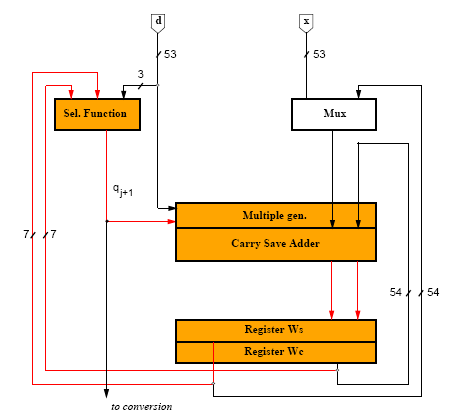
\includegraphics{./noretiming.PNG}
%	\caption{Figure 1: Digit recurrence division}
%	\label{fig:noretiming}
%\end{figure}

%The Sel. function -block implements the quotient digit selection function. The selection function determines a 4-bit quotient digit using 3 most significant bits of the divisor d and 7 most significant bits from the results stored in registers Ws and Wc.

%The MUX block selects the input for the divisor multiplication between the dividend, which is used only in the initialization phase of the division algorithm, and the result of the substraction of the quotient digit/divisor multiplication result from the dividend. The substraction result is stored in register Ws.

%The Multiple gen. -block implements the divisor multiplication ie. it multiplies the divisor d with the 4-bit quotient digit. This block is basically a multiplexer.

%The Carry Save Adder -block implements the substraction of the result of the divisor multiplication from the dividend. The substraction is done with a carry-save adder as the name of the block suggests.

%The registers Ws and Wc store the carry and the sum from the carry-save adder respectively.

%The critical path of this circuit is marked with red arrows in the figure 1.

%\subsection{Design for Division using Retiming}
%explain in detail the circuit for division using retiming. we should argue what is expected from this, and how we should be able to save power in this.
%The retimed design is presented in figure 2.

%\begin{figure}
%	\centering
%		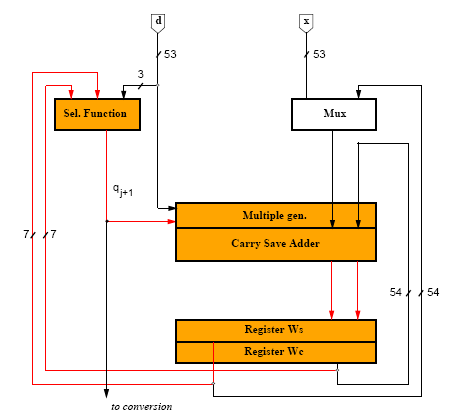
\includegraphics{./noretiming.PNG}
%	\caption{Figure 1: Digit recurrence division retimed}
%	\label{fig:retiming}
%\end{figure}

%Since only the most significant bits of sum and carry are used in the quotient digit selection it makes sense to separate the most significant bits from the least significant bits to separate structural slices. This is done in the VHDL code by disconnecting the quotient digit selection block from the W registers thus \textit{removing registers from the inputs} and adding new registers to the output of the block. This frees the W registers from the most significant slice. By also separating the implementation of the most significant bits of the adder and the multiplie generation from the implementation for the less significant bits more of the design is freed from the critical path.

%These changes do not affect the functionality of the circuit, but by dividing the implementation to most significant and least significant slices we get two paths. The critical path is marked with red arrows in the figure 2. The delay on the critical path is T(SEL)+T(reg q)+T(mux)+T(CSA). The delay on the non-critical path is at maximum T(reg W)+T(mux)+T(CSA). From this it can be seen that the non critical path has some slack which the synthesizer should be able to use to optimize the least significant slice for power, namely by replacing HS cells with LL cells.


%\subsection{Authors by Section}
%\begin{itemize}
%\item \textit{Rajesh Bachani} 
%\item \textit{Josep Renard} 
%\item \textit{Markku Eerola} 
%\end{itemize}

%\section{Implementation of Division using Retiming}
%\label{section:impl}
%explain specifically the changes that were implemented for using the retimed circuit for division. this could also include parts of the VHDL, but mostly it should concentrate on highlighting the changes in terms of the connections between the components.
%we would not have any section for implementation, giving the code, since there is a lot of code in the whole thing. so we should try and just explain all the changes in the code here only.
%\section{Power Report and Cell Count}
%\label{section:power}
% put the reports from the power analysis of both the designs here. also, give a short recap kind of a table here. also, write about the cells here.

%\section{Discussion}
%\label{section:discussion}
%discuss the report at length here. we should clearly justify the results, by explaining why the SVT cells count has reduced and HVT has increased, and why the cell internal power has reduced. ofcourse this was expected, but nice explanation is needed here. 
%\section{Appendix A: The power reports}
%\label{section:reports}

\end{document}